\documentclass[12pt]{article}
% Margin fixes
\oddsidemargin -0.5in
\evensidemargin -0.5in
\textwidth 7.25in
\topmargin 0.0in

\headheight 0.0pt
\headsep 0.0pt
\voffset 0.0pt
\textheight = 9.0in
\usepackage{amsmath,amssymb,graphicx,float}

\title{Magnetic Torque}
\author{Nathan Grouse\\Lisa Tran}

\newcommand{\eV}{\text{eV}}
\newcommand{\V}{\text{V}}
\newcommand{\A}{\text{A}}

% Start the document!
\newcommand{\documentname}{\textsl{Article}}
\begin{document}
\maketitle

\section{Introduction}
\indent \indent To perform experiments with macroscopic magnets that display similar features of experiments with elementary particles. While this doesn't create a perfect representation - quantization will not be observable - this does an ok job.

\subsection{Apparatus}
\indent \indent A cue ball with a magnet in the center and a rod which sticks out in the direction of its "magnetic dipole", sits in a spherical well that has a hole in the bottom. Air is pumped through the hole so the ball sits on a cushion of air. This well sits inbetween two coils connected in series and powered by some current.

\begin{figure}[H]
\centering
\hspace{-0.0in}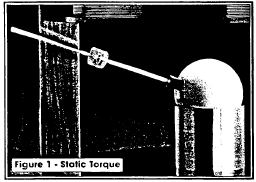
\includegraphics[scale=0.90]{apparatus.png}
\end{figure}

\begin{figure}[H]
\centering
\hspace{-0.0in}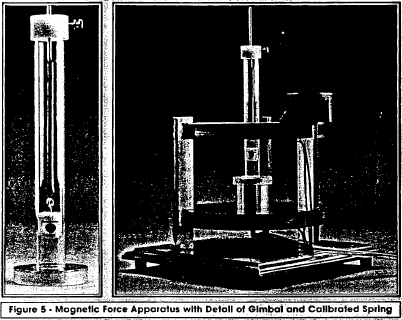
\includegraphics[scale=0.60]{apparatus2.png}
\end{figure}

\section{Theory}
\indent \indent The sections for each of the 4 experiments is sufficiently completed mathematically and the topics were also covered in physics 2 as far the magnetic dipole and torque equations go.

\section{Data}
\begin{figure}[H]
\centering
\hspace{-0.0in}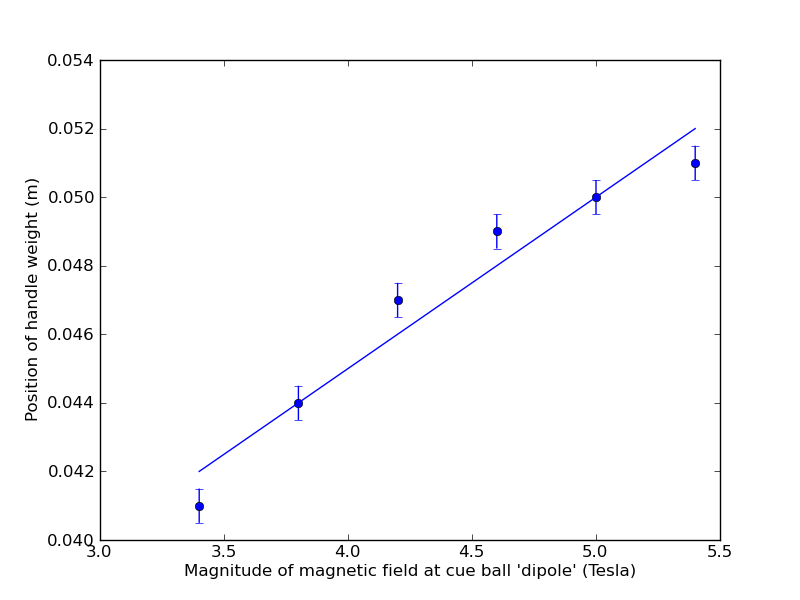
\includegraphics[scale=0.50]{Plot1.png}
\caption{Experiment 1 \label{fig:setup}}
\end{figure}

\begin{figure}[H]
\centering
\hspace{-0.0in}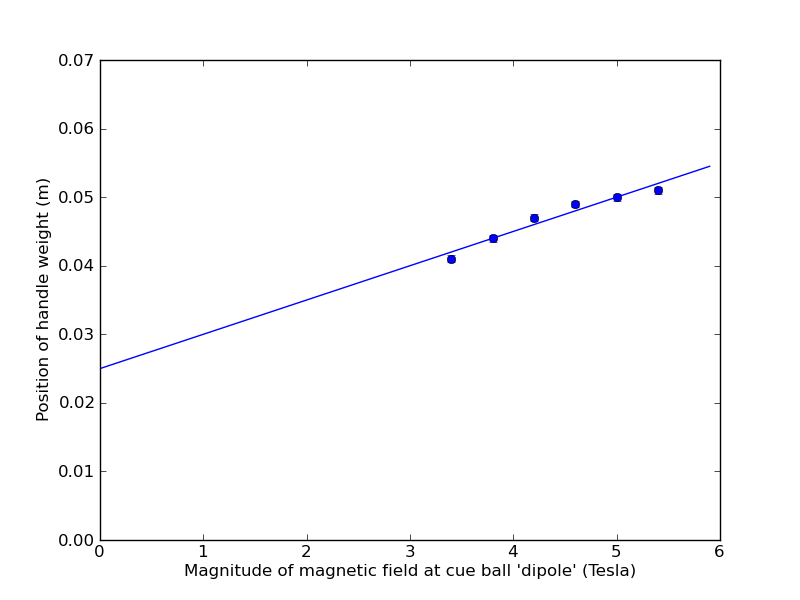
\includegraphics[scale=0.50]{Plot2.png}
\caption{$\frac{\mu}{mg}$ = .005, y-int = .025 \label{fig:setup}}
\end{figure}

\begin{figure}[H]
\centering
\hspace{-0.0in}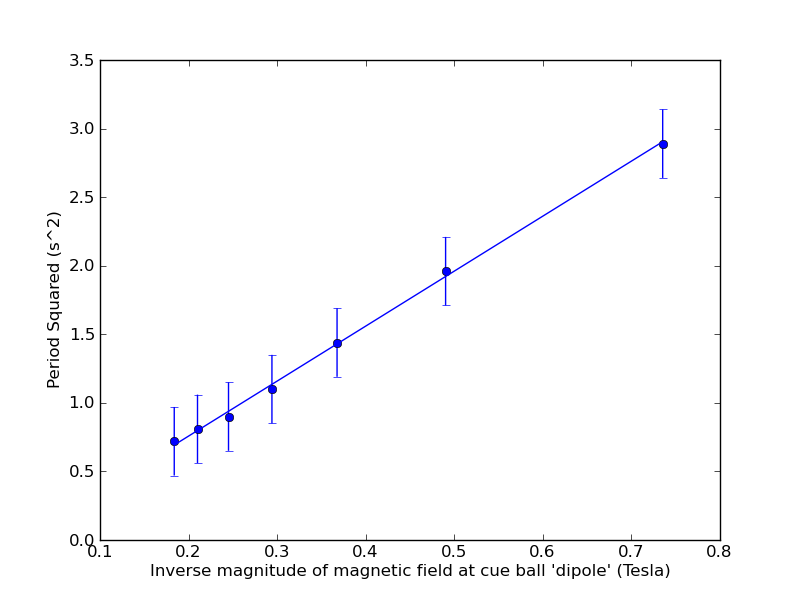
\includegraphics[scale=0.50]{Plot3.png}
\caption{Experiment 2: $\frac{4\pi^2I}{\mu}$ = 4.01 \label{fig:setup}}
\end{figure}

\begin{figure}[H]
\centering
\hspace{-0.0in}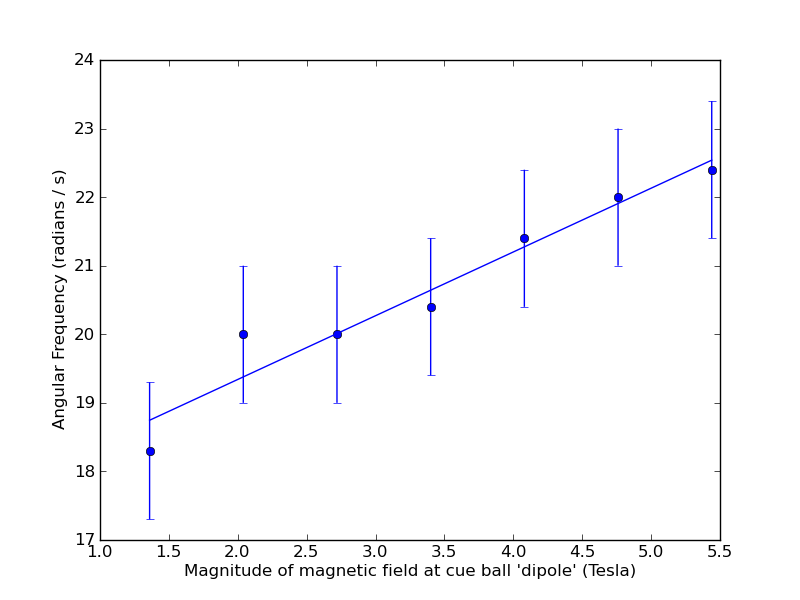
\includegraphics[scale=0.50]{Plot4.png}
\caption{Experiment 3: $\frac{\mu}{L}$ = .93 \label{fig:setup}}
\end{figure}

\begin{figure}[H]
\centering
\hspace{-0.0in}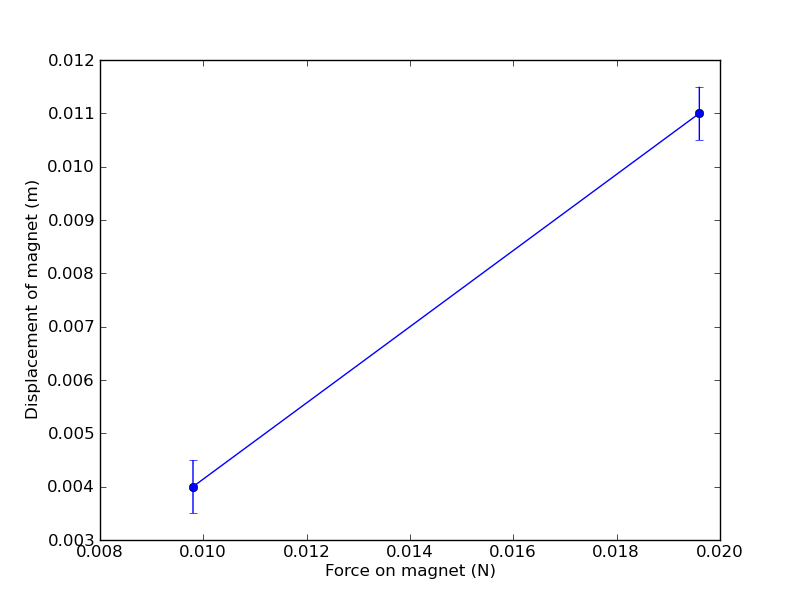
\includegraphics[scale=0.50]{Plot5.png}
\caption{Experiment 4: k = .714 \label{fig:setup}}
\end{figure}

\begin{figure}[H]
\centering
\hspace{-0.0in}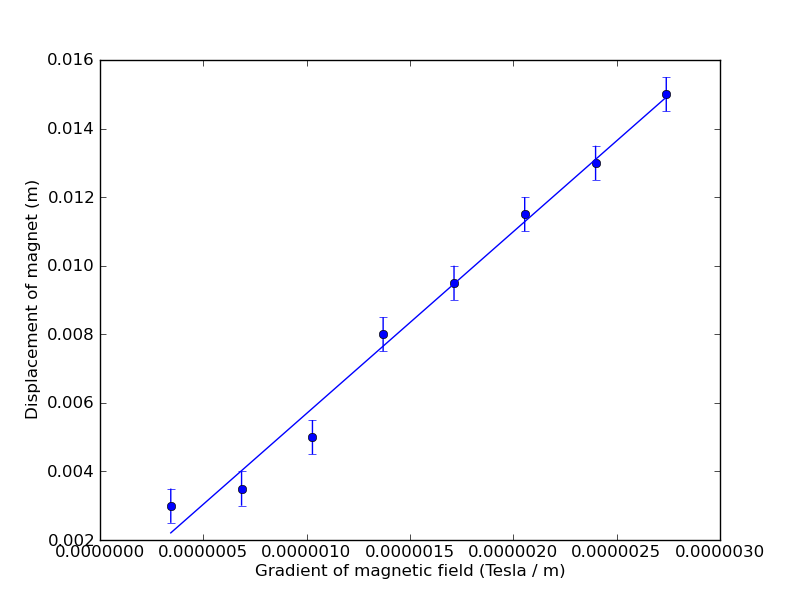
\includegraphics[scale=0.50]{Plot6.png}
\caption{$\frac{\mu}{k}$ = 5300 \label{fig:setup}}
\end{figure}

\section{Calculations}
\indent \indent Experiment 1:
\[\mu = m_w_e_i_g_h_tg*.005 = 7.35 x 10^-^5 \]
\indent Experiment 2:
\[I = \frac{2}{5} m r = 4.056 x 10^-^5 \]
\[ \mu = \frac{4\pi^2I}{4.01} = 3.99 x 10^-^4 \]
\indent Experiment 3:
\[L = I\omega = (4.056 x 10^-^5)(2\pi)(5.1 Hz) = 1.3 x 10^-^3 \frac{kg m^2}{s} \]
\[ \mu = (L)(.93) = 1.2 x 10^-^3 \]
\indent Experiment 4:
\[ \frac{dB}{dz} = 1.69 x 10^-^2 I \frac{Tesla}{meter} (for magnet) = 6.854 x 10^-^7 \frac{Tesla}{meter} \]
\[ k = .714 \]
\[ \mu = (k)(5300) = 3784.2 \]
\indent This last result seems completely off.



\section{Error Analysis}
\indent \indent There was uncertainty of $\pm$ .0005 in measurements for the diamter of the ball and all other values measured with calipers. There was uncertainty of $\pm$ .0001 m in measurements of the length of the ball handle and other values measured with a ruler. There was uncertainty of $\pm$ .00005 kg in measurements of the handle weight and other values measured using the gram scale. There was an uncertainty of .5 s - larger than the precision of the stopwatch to account for human reaction time - in measurements made by the stopwatch. There was an uncertainty of $\pm$ .05 A in measurements of current, determined from the precision of the apparatus. In dermining values for the magnetic field strength, uncertainty in current propagated through a product:

\[ \frac{dq}{|q|} = \sqrt{(\frac{.03 x 10^-^3 Tesla/Ampere}{1.36 Tesla/Ampere})^2 + (\frac{.05 A}{y A})^2} \]


\section{Conclusion}
\indent \indent The results I obtained are sometimes reasonable but not consistent with each other. I'm not sure why the last experiment produced an entirely different order of magnitude result. I think it has something to do with the proportionality of the magnetic field gradient and the current supplied to the apparatus. The relationship wasn't clearly defined in the lab manual so I assumed it was directly proportional, but its entirely possible that this isn't the case.

\section{Questions}
\indent \indent 1. Experiment 4, section a., Observe what happens and write it down. \\
\indent The magnet moves from side to side in teh tube depending on the direction of the magnetic field.

\end{document}